\begin{enumerate}[label=\thesubsection.\arabic*.,ref=\thesubsection.\theenumi]
\item     Balance the following chemical equation.
    \begin{align}
        \label{eq:solutions/chem/6ato balance} HNO_{3}+ Ca(OH)_{2}\to Ca(NO_{3})_{2}+H_{2}O
    \end{align}
\solution
\begin{enumerate}[label=\thesection.\arabic*,ref=\thesection.\theenumi]
\numberwithin{equation}{enumi}
\numberwithin{figure}{enumi}
\numberwithin{table}{enumi}
\item 




\end{enumerate}

%
\item    Balance the following chemical equation.
    \begin{align}
        \label{eq:solutions/chem/7b1} \text{Zinc + Silver nitrate} \to \text{Zinc nitrate + Silver}
    \end{align}
\solution
%NCERT Chapter 10, Circles
\begin{enumerate}[label=\thesection.\arabic*,ref=\thesection.\theenumi]
\numberwithin{equation}{enumi}
\numberwithin{figure}{enumi}
\numberwithin{table}{enumi}
\end{enumerate}

\item Write the balanced chemical equations for the following reaction. 
\begin{align}
 BaCl_2 + K_2SO_4 \rightarrow BaSO_4 + KCl \label{eq:solutions/chemistry/7d:1}   
\end{align}
%\solution
%\begin{enumerate}[label=\thesection.\arabic*,ref=\thesection.\theenumi]
\numberwithin{equation}{enumi}
\numberwithin{figure}{enumi}
\numberwithin{table}{enumi}
\item 
\label{chapters/9/9/3/1}
\begin{align}
	\myvec{3&-4}\vec{x}=\myvec{3&-4}\myvec{-2\\3}
	=-18 
\end{align}
is the required equation of the line.


\item 
\label{chapters/9/9/3/2}
\iffalse
\documentclass[journal,10pt,twocolumn]{article}
\usepackage{graphicx}
\usepackage[margin=0.5in]{geometry}
\usepackage{amsmath}
\usepackage{array}
\usepackage{booktabs}
\usepackage{listings}
\providecommand{\norm}[1]{\left\lVert#1\right\rVert}
\providecommand{\abs}[1]{\left\vert#1\right\vert}
\usepackage{enumerate}
\let\vec\mathbf
\newcommand{\myvec}[1]{\ensuremath{\begin{pmatrix}#1\end{pmatrix}}}
\newcommand{\mydet}[1]{\ensuremath{\begin{vmatrix}#1\end{vmatrix}}}
\providecommand{\brak}[1]{\ensuremath{\left(#1\right)}}
\lstset{
frame=single,
breaklines=true,
columns=fullflexible
}
\title{\textbf{Matrix Assignment}}
\author{ALURU AJAY}
\date{September 2022}
\begin{document}
\maketitle

\section{Problem Statement}
\fi
In $\triangle ABC, \vec{E}$ is the mid-point of median $AD$.
Show that 
\begin{align}
ar(\triangle BED) = \frac{1}{4} ar(\triangle ABC)
		\label{eq:9/9/3/2}
\end{align}
	\begin{figure}[H]
		\centering
 \includegraphics[width=0.75\columnwidth]{chapters/9/9/3/2/figs/fig_Triangle.png}
		\caption{}
		\label{fig:9/9/3/2}
  	\end{figure}
\begin{proof}
	From Problem 
\ref{chapters/9/9/3/2},
  \begin{align}
ar(\triangle BED) =
 \frac{1}{4}\norm{\vec{B} \times \vec{C}+\vec{C} \times \vec{E}+\vec{E} \times \vec{B}}
		\label{eq:9/9/3/2/1}
  \end{align}
  Since 
  \begin{align}
	  \vec{E} &= \frac{ \vec{A}+\vec{D}}{2}
	  \\
	  &= \frac{ 2\vec{A}+\vec{B} + \vec{C}}{4},
  \end{align}
  substituting the above in 
		\eqref{eq:9/9/3/2/1}
		yields
  \begin{align}
	  ar(\triangle BED) &=
 \frac{1}{4}\norm{\vec{B} \times \vec{C}+\vec{C} \times \frac{ 2\vec{A}+\vec{B} + \vec{C}}{4}+\frac{ 2\vec{A}+\vec{B} + \vec{C}}{4} \times \vec{B}}
 \\
	  &=\frac{1}{8}\norm{\vec{A} \times \vec{B}+\vec{B} \times \vec{C}+\vec{C} \times \vec{A}}
  \end{align}
  resulting in
		\eqref{eq:9/9/3/2}.
\end{proof}
\iffalse

\section{Diagram}
Plot of Triangle is shown in figure 1, where point B is origin and points A, B, C and D are the vertices of Triangle.
\begin{figure}[H]
\includegraphics[width=0.75\columnwidth]{fig_Triangle.png}
\caption{Triangle}
\label{fig:Triangle}
\end{figure}
\section{PROOF}
In $\Delta ABC$,with AD as median
E is the mid-point of AD
\begin{center}
    $||{\vec{E-A}}||$ = $||{\vec{E-D}}||$
\end{center}
\begin{center}
\begin{equation}
    ||{\vec{D-B}}|| = \frac{1}{2} ||{\vec{C-B}}||
\end{equation}
\end{center}
\begin{flushleft}
From $\Delta ABC$
\end{flushleft}
\begin{equation}
    ar(\Delta ABC) = \frac{1}{2} \times ||{\vec{B-A}}|| \times ||{\vec{C-B}}||
\end{equation}
\begin{flushleft}
From $\Delta BED$
\vspace{0.3cm}\\
ar($\Delta BED$) = $\frac{1}{2}$ $\times$ $||{\vec{E-B}}||$ $\times$ $||{\vec{D-B}}||$
\vspace{0.3cm}\\
From Eq(1) we can write as
\begin{equation}
    ar(\Delta BED) = \frac{1}{2} \times ||{\vec{E-B}}|| \times\frac{1}{2} ||{\vec{C-B}}||
\end{equation}
We know that from Parallelogram law of Vector Addition
\begin{equation}
     \vec{E-B} = \frac{1}{2} ((\vec{B-A}) + \vec{C-B}))
\end{equation}
Substituting Eq(4) in Eq(3) $\And$ re-writing the Eq(3)\\
\vspace{0.3cm}
ar($\Delta BED$) = $\frac{1}{2}$ $\times$ (($\frac{1}{2}$$||{\vec{(B-A) + (C-B)}}||$) $\times$$\frac{1}{2}$ $||{\vec{C-B}}||$)
\vspace{0.5cm}\\
ar($\Delta BED$) = $\frac{1}{2}$ $\times$ $\frac{1}{4}$($||{\vec{B-A}}||$ $\times$ $||{\vec{C-B}}||$)
\vspace{0.5cm}\\
ar($\Delta BED$) =$\frac{1}{4}$ ($\frac{1}{2}$ $\times$ $||{\vec{B-A}}||$ $\times$ $||{\vec{C-B}}||$)
\vspace{0.5cm}\\
From Eq(2)
\vspace{0.3cm}\\
ar($\Delta BED$) =$\frac{1}{4}$(ar($\Delta ABC$)
\end{flushleft}
\vspace{0.5cm}
\centering
\begin{tabular}{|c|}
\hline
Ar($\Delta$ BED) = $\frac{1}{4}$ Ar($\Delta$ ABC)\\
\hline
\end{tabular}\\
\vspace{0.5cm}
Hence Proved

\begin{flushleft}
\section{Software}
\end{flushleft}
Download the codes given in the link below and execute them.\\
\begin{table}[H]
\centering
\begin{tabular}{|c|} \hline
\rule{0pt}{10pt} 
https://raw.githubusercontent.com/19PA1AO410/\\
FWC-Module-1/main/Matrix%20_Assignment/line_assignment/line.py
\\\hline
 \end{tabular}
\end{table}
\bibliographystyle{ieeetr}
\end{document}
\end{document}
\fi

\item 
\label{chapters/9/9/3/3}
\begin{align}
	\myvec{3&-4}\vec{x}=\myvec{3&-4}\myvec{-2\\3}
	=-18 
\end{align}
is the required equation of the line.

\item 
\label{chapters/9/9/3/4}
\begin{align}
	\myvec{3&-4}\vec{x}=\myvec{3&-4}\myvec{-2\\3}
	=-18 
\end{align}
is the required equation of the line.

\item 
\item 
\item 
\item 

\item 
\label{chapters/9/9/3/9}
\begin{align}
	\myvec{3&-4}\vec{x}=\myvec{3&-4}\myvec{-2\\3}
	=-18 
\end{align}
is the required equation of the line.


\item 
\item 
\label{chapters/9/9/3/11}
\begin{align}
	\myvec{3&-4}\vec{x}=\myvec{3&-4}\myvec{-2\\3}
	=-18 
\end{align}
is the required equation of the line.

\item 
\item 
\item 
\item 
\item 
\label{chapters/9/9/3/16}
\begin{align}
	\myvec{3&-4}\vec{x}=\myvec{3&-4}\myvec{-2\\3}
	=-18 
\end{align}
is the required equation of the line.

\iffalse
\item 
\label{chapters/9/9/3/4}
\begin{align}
	\myvec{3&-4}\vec{x}=\myvec{3&-4}\myvec{-2\\3}
	=-18 
\end{align}
is the required equation of the line.

\item 
\label{chapters/9/9/3/4}
\begin{align}
	\myvec{3&-4}\vec{x}=\myvec{3&-4}\myvec{-2\\3}
	=-18 
\end{align}
is the required equation of the line.

\item 
\label{chapters/9/9/3/4}
\begin{align}
	\myvec{3&-4}\vec{x}=\myvec{3&-4}\myvec{-2\\3}
	=-18 
\end{align}
is the required equation of the line.

\item 
\label{chapters/9/9/3/4}
\begin{align}
	\myvec{3&-4}\vec{x}=\myvec{3&-4}\myvec{-2\\3}
	=-18 
\end{align}
is the required equation of the line.

\item 
\label{chapters/9/9/3/4}
\begin{align}
	\myvec{3&-4}\vec{x}=\myvec{3&-4}\myvec{-2\\3}
	=-18 
\end{align}
is the required equation of the line.

\item 
\label{chapters/9/9/3/4}
\begin{align}
	\myvec{3&-4}\vec{x}=\myvec{3&-4}\myvec{-2\\3}
	=-18 
\end{align}
is the required equation of the line.

\item 
\label{chapters/9/9/3/4}
\begin{align}
	\myvec{3&-4}\vec{x}=\myvec{3&-4}\myvec{-2\\3}
	=-18 
\end{align}
is the required equation of the line.

\fi

\end{enumerate}

\item Balance the following chemical equation.
%
\begin{align}
\label{eq:chem_balance}
Fe+H_2O &\rightarrow Fe_3O_4 + H_2
\end{align}
%\solution 
%\begin{enumerate}[label=\thesection.\arabic*,ref=\thesection.\theenumi]
\numberwithin{equation}{enumi}
\numberwithin{figure}{enumi}
\numberwithin{table}{enumi}
\item 
\item 
\item 
\label{chapters/9/9/4/3}
\begin{align}
	\myvec{3&-4}\vec{x}=\myvec{3&-4}\myvec{-2\\3}
	=-18 
\end{align}
is the required equation of the line.


\item 
\label{chapters/9/9/4/4}
\begin{align}
	\myvec{3&-4}\vec{x}=\myvec{3&-4}\myvec{-2\\3}
	=-18 
\end{align}
is the required equation of the line.

\item 
\label{chapters/9/9/4/5}
\begin{align}
	\myvec{3&-4}\vec{x}=\myvec{3&-4}\myvec{-2\\3}
	=-18 
\end{align}
is the required equation of the line.

\item 
\item 
\item 
\end{enumerate}

\item Balance the following chemical equation.
\begin{align}
  \label{matrix/50/eq1}
NaOH + H_2SO_4 \xrightarrow{} Na_2SO_4  +  H_2O
\end{align}
%\\
%\solution
%\input{chapters/chemistry/solutions/5.tex}
%\item Balance the following chemical equation
%\begin{align}\label{1}
%    BaCl_2 + H_2SO_4 \xrightarrow{} BaSO_4 + HCl
%\end{align}
\end{enumerate}
 

